\definecolor{c1}{rgb}{0 0.4470 0.7410}
\definecolor{c2}{rgb}{0.8500 0.3250 0.0980}
\definecolor{c3}{rgb}{0.9290 0.6940 0.1250}
\definecolor{c4}{rgb}{0.4940 0.1840 0.5560}
\definecolor{c5}{rgb}{0.4660 0.6740 0.1880}
\definecolor{c9}{RGB}{255,0,255}

% GNUPLOT: LaTeX picture with Postscript
\begingroup
  \makeatletter
  \providecommand\color[2][]{%
    \GenericError{(gnuplot) \space\space\space\@spaces}{%
      Package color not loaded in conjunction with
      terminal option `colourtext'%
    }{See the gnuplot documentation for explanation.%
    }{Either use 'blacktext' in gnuplot or load the package
      color.sty in LaTeX.}%
    \renewcommand\color[2][]{}%
  }%
  \providecommand\includegraphics[2][]{%
    \GenericError{(gnuplot) \space\space\space\@spaces}{%
      Package graphicx or graphics not loaded%
    }{See the gnuplot documentation for explanation.%
    }{The gnuplot epslatex terminal needs graphicx.sty or graphics.sty.}%
    \renewcommand\includegraphics[2][]{}%
  }%
  \providecommand\rotatebox[2]{#2}%
  \@ifundefined{ifGPcolor}{%
    \newif\ifGPcolor
    \GPcolorfalse
  }{}%
  \@ifundefined{ifGPblacktext}{%
    \newif\ifGPblacktext
    \GPblacktexttrue
  }{}%
  % define a \g@addto@macro without @ in the name:
  \let\gplgaddtomacro\g@addto@macro
  % define empty templates for all commands taking text:
  \gdef\gplfronttext{}%
  \gdef\gplfronttext{}%
  \makeatother
  \ifGPblacktext
    % no textcolor at all
    \def\colorrgb#1{}%
    \def\colorgray#1{}%
  \else
    % gray or color?
    \ifGPcolor
      \def\colorrgb#1{\color[rgb]{#1}}%
      \def\colorgray#1{\color[gray]{#1}}%
      \expandafter\def\csname LTw\endcsname{\color{white}}%
      \expandafter\def\csname LTb\endcsname{\color{black}}%
      \expandafter\def\csname LTa\endcsname{\color{black}}%
      \expandafter\def\csname LT0\endcsname{\color[rgb]{1,0,0}}%
      \expandafter\def\csname LT1\endcsname{\color[rgb]{0,1,0}}%
      \expandafter\def\csname LT2\endcsname{\color[rgb]{0,0,1}}%
      \expandafter\def\csname LT3\endcsname{\color[rgb]{1,0,1}}%
      \expandafter\def\csname LT4\endcsname{\color[rgb]{0,1,1}}%
      \expandafter\def\csname LT5\endcsname{\color[rgb]{1,1,0}}%
      \expandafter\def\csname LT6\endcsname{\color[rgb]{0,0,0}}%
      \expandafter\def\csname LT7\endcsname{\color[rgb]{1,0.3,0}}%
      \expandafter\def\csname LT8\endcsname{\color[rgb]{0.5,0.5,0.5}}%
    \else
      % gray
      \def\colorrgb#1{\color{black}}%
      \def\colorgray#1{\color[gray]{#1}}%
      \expandafter\def\csname LTw\endcsname{\color{white}}%
      \expandafter\def\csname LTb\endcsname{\color{black}}%
      \expandafter\def\csname LTa\endcsname{\color{black}}%
      \expandafter\def\csname LT0\endcsname{\color{black}}%
      \expandafter\def\csname LT1\endcsname{\color{black}}%
      \expandafter\def\csname LT2\endcsname{\color{black}}%
      \expandafter\def\csname LT3\endcsname{\color{black}}%
      \expandafter\def\csname LT4\endcsname{\color{black}}%
      \expandafter\def\csname LT5\endcsname{\color{black}}%
      \expandafter\def\csname LT6\endcsname{\color{black}}%
      \expandafter\def\csname LT7\endcsname{\color{black}}%
      \expandafter\def\csname LT8\endcsname{\color{black}}%
    \fi
  \fi
    \setlength{\unitlength}{0.0500bp}%
    \ifx\gptboxheight\undefined%
      \newlength{\gptboxheight}%
      \newlength{\gptboxwidth}%
      \newsavebox{\gptboxtext}%
    \fi%
    \setlength{\fboxrule}{0.5pt}%
    \setlength{\fboxsep}{1pt}%
\begin{picture}(8000.00,12000.00)%
    \gplgaddtomacro\gplfronttext{%
      \colorrgb{0.15,0.15,0.15}%
      \put(908,10069){\makebox(0,0)[r]{\strut{}$0.0$}}%
      \colorrgb{0.15,0.15,0.15}%
      \put(908,10241){\makebox(0,0)[r]{\strut{}$0.05$}}%
      \colorrgb{0.15,0.15,0.15}%
      \put(908,10412){\makebox(0,0)[r]{\strut{}$0.10$}}%
      \colorrgb{0.15,0.15,0.15}%
      \put(908,10584){\makebox(0,0)[r]{\strut{}$0.15$}}%
      \colorrgb{0.15,0.15,0.15}%
      \put(908,10756){\makebox(0,0)[r]{\strut{}$0.20$}}%
      \colorrgb{0.15,0.15,0.15}%
      \put(908,10927){\makebox(0,0)[r]{\strut{}$0.25$}}%
      \colorrgb{0.15,0.15,0.15}%
      \put(908,11099){\makebox(0,0)[r]{\strut{}$0.30$}}%
    }%
    \gplgaddtomacro\gplfronttext{%
      \colorrgb{0.00,0.00,0.00}%
      \put(4000,12219){\makebox(0,0){\strut{}Κατανομές σφαλμάτων θέσης [m]}}%
      \put(1000,11719){\makebox(0,0){\strut{}{\color{c1}{\rule[0.6mm]{0.5cm}{0.5mm}}}\small PLICP}}
      \put(2000,11719){\makebox(0,0){\strut{}{\color{c2}{\rule[0.6mm]{0.5cm}{0.5mm}}}\small NDT}}
      \put(3000,11719){\makebox(0,0){\strut{}{\color{c3}{\rule[0.6mm]{0.5cm}{0.5mm}}}\small FastGICP}}
      \put(4400,11719){\makebox(0,0){\strut{}{\color{c4}{\rule[0.6mm]{0.5cm}{0.5mm}}}\small FastVGICP}}
      \put(5800,11719){\makebox(0,0){\strut{}{\color{c5}{\rule[0.6mm]{0.5cm}{0.5mm}}}\small NDT-PSO}}
      \put(6900,11719){\makebox(0,0){\strut{}{\color{c9}{\rule[0.6mm]{0.5cm}{0.5mm}}}\small \texttt{fsm}}}
      \put(4139,11219){\makebox(0,0){\strut{}\scriptsize $(\overline{\delta}_{xy}, \overline{\delta}_\theta) = (0.05 \ \text{m}, 0.035 \ \text{rad})$}}%
    }%
    \gplgaddtomacro\gplfronttext{%
      \colorrgb{0.15,0.15,0.15}%
      \put(908,8669){\makebox(0,0)[r]{\strut{}\small $0.0$}}%
      \colorrgb{0.15,0.15,0.15}%
      \put(908,8841){\makebox(0,0)[r]{\strut{}\small $0.05$}}%
      \colorrgb{0.15,0.15,0.15}%
      \put(908,9012){\makebox(0,0)[r]{\strut{}\small $0.10$}}%
      \colorrgb{0.15,0.15,0.15}%
      \put(908,9184){\makebox(0,0)[r]{\strut{}\small $0.15$}}%
      \colorrgb{0.15,0.15,0.15}%
      \put(908,9356){\makebox(0,0)[r]{\strut{}\small $0.20$}}%
      \colorrgb{0.15,0.15,0.15}%
      \put(908,9527){\makebox(0,0)[r]{\strut{}\small $0.25$}}%
      \colorrgb{0.15,0.15,0.15}%
      \put(908,9699){\makebox(0,0)[r]{\strut{}\small $0.30$}}%
    }%
    \gplgaddtomacro\gplfronttext{%
      \colorrgb{0.00,0.00,0.00}%
      \put(4139,9819){\makebox(0,0){\strut{}\scriptsize $(\overline{\delta}_{xy}, \overline{\delta}_\theta) = (0.10 \ \text{m}, 0.070 \ \text{rad})$}}%
    }%
    \gplgaddtomacro\gplfronttext{%
      \colorrgb{0.15,0.15,0.15}%
      \put(908,7269){\makebox(0,0)[r]{\strut{}\small $0.0$}}%
      \colorrgb{0.15,0.15,0.15}%
      \put(908,7416){\makebox(0,0)[r]{\strut{}\small $0.05$}}%
      \colorrgb{0.15,0.15,0.15}%
      \put(908,7563){\makebox(0,0)[r]{\strut{}\small $0.10$}}%
      \colorrgb{0.15,0.15,0.15}%
      \put(908,7710){\makebox(0,0)[r]{\strut{}\small $0.15$}}%
      \colorrgb{0.15,0.15,0.15}%
      \put(908,7858){\makebox(0,0)[r]{\strut{}\small $0.20$}}%
      \colorrgb{0.15,0.15,0.15}%
      \put(908,8005){\makebox(0,0)[r]{\strut{}\small $0.25$}}%
      \colorrgb{0.15,0.15,0.15}%
      \put(908,8152){\makebox(0,0)[r]{\strut{}\small $0.30$}}%
      \colorrgb{0.15,0.15,0.15}%
      \put(908,8299){\makebox(0,0)[r]{\strut{}\small $0.35$}}%
    }%
    \gplgaddtomacro\gplfronttext{%
      \colorrgb{0.15,0.15,0.15}%
      \colorrgb{0.00,0.00,0.00}%
      \put(4139,8419){\makebox(0,0){\strut{}\scriptsize $(\overline{\delta}_{xy}, \overline{\delta}_\theta) = (0.15 \ \text{m}, 0.15 \ \text{rad})$}}%
    }%
    \gplgaddtomacro\gplfronttext{%
      \colorrgb{0.15,0.15,0.15}%
      \put(908,5869){\makebox(0,0)[r]{\strut{}\small $0.0$}}%
      \colorrgb{0.15,0.15,0.15}%
      \put(908,6016){\makebox(0,0)[r]{\strut{}\small $0.05$}}%
      \colorrgb{0.15,0.15,0.15}%
      \put(908,6163){\makebox(0,0)[r]{\strut{}\small $0.10$}}%
      \colorrgb{0.15,0.15,0.15}%
      \put(908,6310){\makebox(0,0)[r]{\strut{}\small $0.15$}}%
      \colorrgb{0.15,0.15,0.15}%
      \put(908,6458){\makebox(0,0)[r]{\strut{}\small $0.20$}}%
      \colorrgb{0.15,0.15,0.15}%
      \put(908,6605){\makebox(0,0)[r]{\strut{}\small $0.25$}}%
      \colorrgb{0.15,0.15,0.15}%
      \put(908,6752){\makebox(0,0)[r]{\strut{}\small $0.30$}}%
      \colorrgb{0.15,0.15,0.15}%
      \put(908,6899){\makebox(0,0)[r]{\strut{}\small $0.35$}}%
    }%
    \gplgaddtomacro\gplfronttext{%
      \colorrgb{0.00,0.00,0.00}%
      \put(4139,7019){\makebox(0,0){\strut{}\scriptsize $(\overline{\delta}_{xy}, \overline{\delta}_\theta) = (0.20 \ \text{m}, 0.30 \ \text{rad})$}}%
    }%
    \gplgaddtomacro\gplfronttext{%
      \colorrgb{0.15,0.15,0.15}%
      \put(908,4469){\makebox(0,0)[r]{\strut{}\small $0.0$}}%
      \colorrgb{0.15,0.15,0.15}%
      \put(908,4616){\makebox(0,0)[r]{\strut{}\small $0.05$}}%
      \colorrgb{0.15,0.15,0.15}%
      \put(908,4763){\makebox(0,0)[r]{\strut{}\small $0.10$}}%
      \colorrgb{0.15,0.15,0.15}%
      \put(908,4910){\makebox(0,0)[r]{\strut{}\small $0.15$}}%
      \colorrgb{0.15,0.15,0.15}%
      \put(908,5058){\makebox(0,0)[r]{\strut{}\small $0.20$}}%
      \colorrgb{0.15,0.15,0.15}%
      \put(908,5205){\makebox(0,0)[r]{\strut{}\small $0.25$}}%
      \colorrgb{0.15,0.15,0.15}%
      \put(908,5352){\makebox(0,0)[r]{\strut{}\small $0.30$}}%
      \colorrgb{0.15,0.15,0.15}%
      \put(908,5499){\makebox(0,0)[r]{\strut{}\small $0.35$}}%
    }%
    \gplgaddtomacro\gplfronttext{%
      \colorrgb{0.00,0.00,0.00}%
      \put(4139,5619){\makebox(0,0){\strut{}\scriptsize $(\overline{\delta}_{xy}, \overline{\delta}_\theta) = (0.20 \ \text{m}, 0.56 \ \text{rad})$}}%
    }%
    \gplgaddtomacro\gplfronttext{%
      \colorrgb{0.15,0.15,0.15}%
      \put(908,3069){\makebox(0,0)[r]{\strut{}\small $0.0$}}%
      \colorrgb{0.15,0.15,0.15}%
      \put(908,3216){\makebox(0,0)[r]{\strut{}\small $0.05$}}%
      \colorrgb{0.15,0.15,0.15}%
      \put(908,3363){\makebox(0,0)[r]{\strut{}\small $0.10$}}%
      \colorrgb{0.15,0.15,0.15}%
      \put(908,3510){\makebox(0,0)[r]{\strut{}\small $0.15$}}%
      \colorrgb{0.15,0.15,0.15}%
      \put(908,3658){\makebox(0,0)[r]{\strut{}\small $0.20$}}%
      \colorrgb{0.15,0.15,0.15}%
      \put(908,3805){\makebox(0,0)[r]{\strut{}\small $0.25$}}%
      \colorrgb{0.15,0.15,0.15}%
      \put(908,3952){\makebox(0,0)[r]{\strut{}\small $0.30$}}%
      \colorrgb{0.15,0.15,0.15}%
      \put(908,4099){\makebox(0,0)[r]{\strut{}\small $0.35$}}%
      \colorrgb{0.15,0.15,0.15}%
      \put(1660,2849){\makebox(0,0){\strut{}$0.01$}}%
      \colorrgb{0.15,0.15,0.15}%
      \put(2900,2849){\makebox(0,0){\strut{}$0.03$}}%
      \colorrgb{0.15,0.15,0.15}%
      \put(4140,2849){\makebox(0,0){\strut{}$0.05$}}%
      \colorrgb{0.15,0.15,0.15}%
      \put(5379,2849){\makebox(0,0){\strut{}$0.10$}}%
      \colorrgb{0.15,0.15,0.15}%
      \put(6619,2849){\makebox(0,0){\strut{}$0.20$}}%
    }%
    \gplgaddtomacro\gplfronttext{%
      \colorrgb{0.15,0.15,0.15}%
      \put(4139,2519){\makebox(0,0){\strut{}Τυπική απόκλιση διαταραχών $\sigma_R$ [m]}}%
      \colorrgb{0.00,0.00,0.00}%
      \put(4139,4219){\makebox(0,0){\strut{}\scriptsize $(\overline{\delta}_{xy}, \overline{\delta}_\theta) = (0.20 \ \text{m}, \pi/4 \ \text{rad})$}}%
    }%
    \put(0,0){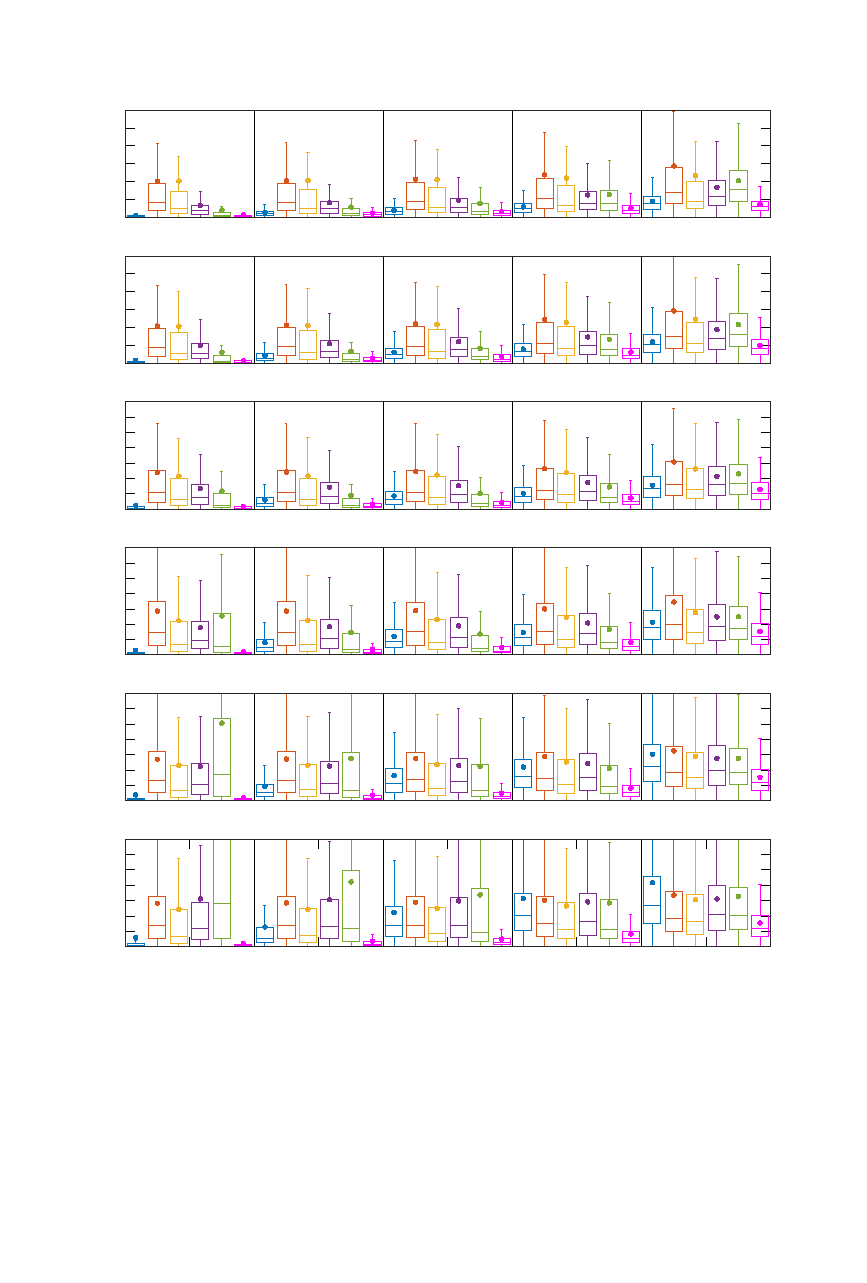
\includegraphics{./figures/parts/02/chapters/05/sections/03/position_errors}}%
    \gplfronttext
  \end{picture}%
\endgroup
